% year: 2026
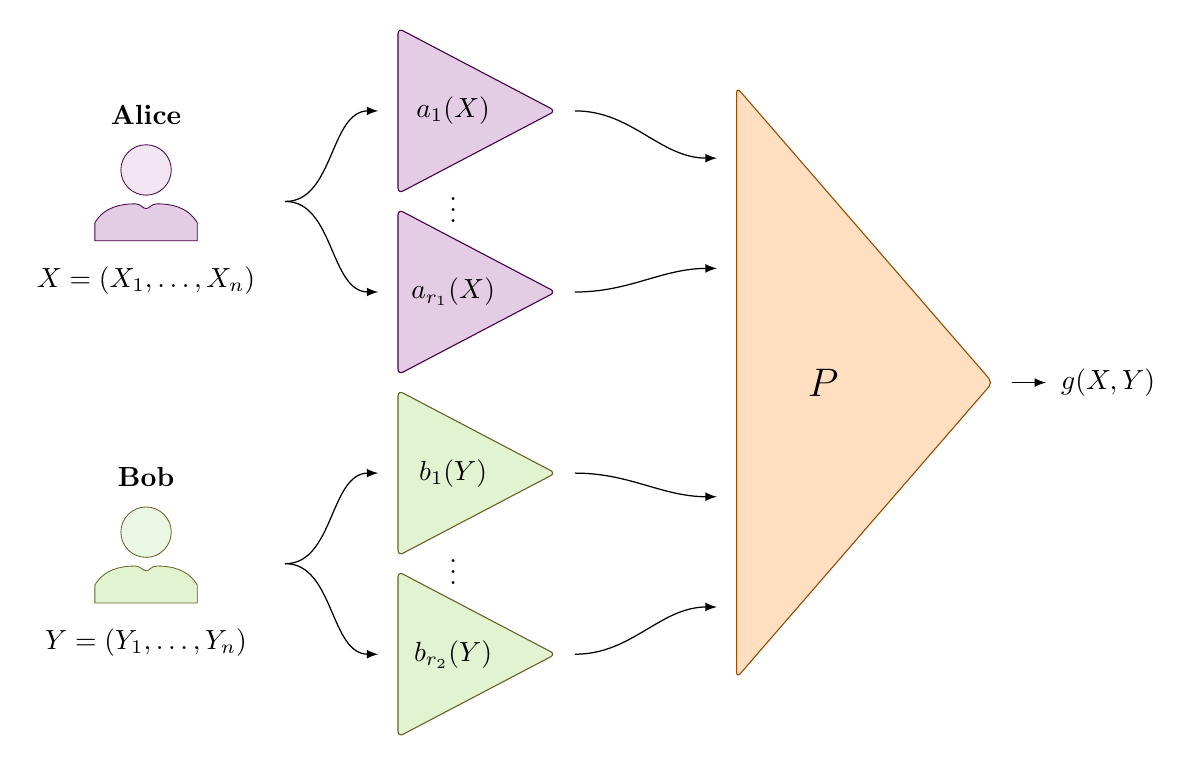
\begin{tikzpicture}[line width=.3pt,line cap=round,line join=round,
  flow/.style={-latex,line width=.45pt,shorten <=2pt,shorten >=2pt},
  computation/.style={rounded corners=2pt,line width=.4pt}]
  \foreach \offset/\party/\inputvar/\messagevar/\partyindex/\headfill/\bodyfill/\outline in {
    0/Alice/X/a/1/violet!10/violet!20/violet!55!black,
    -4.6/Bob/Y/b/2/yellow!20!green!10/yellow!35!green!18/olive!65!black} {
    \begin{scope}[yshift=\offset cm,
      local/.style={draw=\outline,fill=\bodyfill}]
      \node[font=\bfseries] at (1.5,-2.35) {\party};
      \draw[local,fill=\headfill] (1.5,-3.05) circle (.32);
      \draw[local]
        (.85,-3.95) -- (.85,-3.72)
        .. controls (.97,-3.52) and (1.18,-3.48) .. (1.36,-3.48)
        .. controls (1.44,-3.48) and (1.45,-3.54) .. (1.5,-3.54)
        .. controls (1.55,-3.54) and (1.56,-3.48) .. (1.64,-3.48)
        .. controls (1.82,-3.48) and (2.03,-3.52) .. (2.15,-3.72)
        -- (2.15,-3.95) -- cycle;
      \node at (1.5,-4.45) {$\inputvar=(\inputvar_1,\ldots,\inputvar_n)$};
      \foreach \index/\pos in {1/-2.3,{r_{\partyindex}}/-4.6} {
        \draw[computation,local]
          (4.7,{\pos+1.05}) -- (4.7,{\pos-1.05}) -- (6.7,\pos) -- cycle;
        \node at (5.4,\pos) {$\messagevar_{\index}(\inputvar)$};
        \draw[flow] (3.2,-3.45) to[out=0,in=180] (4.52,\pos);
      }
      \node at (5.4,-3.45) {$\vdots$};
    \end{scope}
  }
  \draw[computation,draw=orange!60!black,fill=orange!25]
    (9,-2) -- (9,-9.5) -- (12.25,-5.75) -- cycle;
  \node[font=\Large] at (10.1,-5.75) {$P$};
  \foreach \starty/\endy in {-2.3/-2.9,-4.6/-4.3,-6.9/-7.2,-9.2/-8.6}
    \draw[flow] (6.88,\starty) to[out=0,in=180] (8.82,\endy);
  \node[anchor=west] (gout) at (13,-5.75) {$g(X,Y)$};
  \draw[flow] (12.43,-5.75) -- (gout.west);
\end{tikzpicture}
